\section{Нейронные сети}
	Искуственная нейронная сеть - это математическая модель, построенная по принципу организации и функционирования биологических нейронных сетей. Она представляет из себя систему соединенных простых блоков - искуственных нейронов - каждый из которых имеет входы и выходы для взаимодействия с другими нейронами. Главное преимущество нейронных сетей перед традиционными алгоритмами в том, что они обучаются на некотором наборе данных, а не программируются в классическом смысле этого понятия. Процесс обучения заключается в нахождении оптимальных весовых коэффициентов между нейронами. С математической точки зрения, процесс обучения - это задача многопараметрической нелинейной оптимизации.
	\subsection{Математическая модель нейрона}
		Одиночный нейрон обычно представляет собой взвешенный сумматор с нелинейной функцией активации на выходе (Рис. \ref{artificial-neuron-model}):
		$$x_{out} = \phi(\vec{w} \cdotp \vec{x_{in}}),$$
		где $\vec{w}$ - вектор весовых коэффициентов связей, $\vec{x_{in}}$ - входной вектор, $\phi$ - нелинейная функция активации.
		\begin{figure}[h]
			\begin{center}
				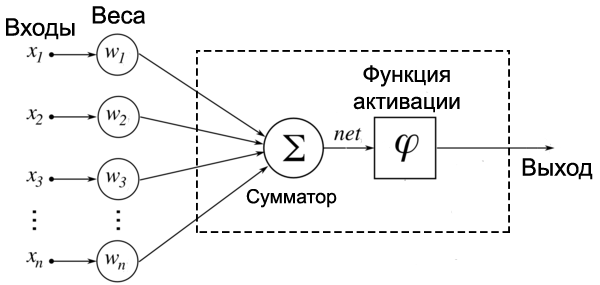
\includegraphics[width=0.7\linewidth]{artificialneuronmodel}
			\end{center}
			\caption{Математическая модель нейрона}
			\label{artificial-neuron-model}
		\end{figure}
		
		Функция активации может выбираться разной в зависимости от задачи. Наиболее часто используемые функции:
		\begin{itemize}
			\item Сигмоида (логистическая функция)
					$$\sigma(x) = \frac{1}{1 + e^{-x}}$$
			\item Гиперболический тангенс
			\item ReLU
					$$ReLU(x) = \max(0, x)$$
			\item softmax
					$$\sigma(\vec{x})_j = \frac{e^{x_j}}{\sum_{k=1}^{N} e^{z_k}}$$
		\end{itemize}
		Множество таких нейроной объединяется в сеть и обучается каким-либо методом.
	\subsection{Метод обратного распространения ошибки}
		Метод обратного распространения ошибки (backpropagation) - самый широко используемый и успешный алгоритм обучения глубоких (многослойных) нейронных сетей. Суть этого метода заключается в распространении сигналов ошибки от выходов сети к ее входам в обратном к распространению сигнала в сети направлении. Это позволяет вычислить производные ошибки по весам сети, которые потом можно использовать в любом градиентном алгоритме оптимизации (например, в стохастическом градиентном спуске).
		
		Обозначим множество входов сети как $\{x_1, \ldots, x_n\}$, множество выходов - $Out$, $w_{ij}$ - вес, присвоенный ребру, соединяющему i-й и j-й узлы, $y_k$ - известные (правильные) ответы, $o_i$ - выход i-го узла. Введем функцию ошибки (например, сумма квадратов расстояний):
		$$ L(\vec{x}, W) = \frac{1}{2} \sum_{k \in Out} (t_k - o_k)^2, $$
		где $W = \{w_{ij}\}$ - матрица весовых коэффициентов
		
		Рассмотрим сначала нейроны последнего слоя. Весовой коэффициент $w_{ij}$ влияет на выход сети как часть суммы $S_j = \sum_i w_{ij} x_i$. Соответственно
		$$ \frac{\partial L}{\partial w_{ij}} = \frac{\partial L}{\partial S_j} \frac{\partial S_j}{\partial w_{ij}} = x_i \frac{\partial L}{\partial S_j} $$
		
		продолжение следует
		
